\documentclass[convert]{standalone}

\usepackage{tikz}
\usepackage{graphicx}
\pagestyle{empty}

% INT_AY22_L29-Fig01_Charges_on_trig.png

\begin{document}
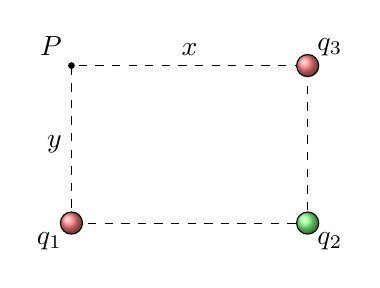
\begin{tikzpicture}

	% Definition
	
	\def\x{3}		% Horizontal extent
	\def\y{2}		% Vertical extent
	
	% Rectangle w/ distance labels
	
	\draw [dashed] (0, 0) -- (\x, 0) -- (\x, \y) -- node [above] {$x$} (0, \y) -- node [left] {$y$} cycle;
	
	% Charges
	
	\draw [ball color = red!50] (0, 0) circle (4 pt) node [below left] {$q_1$};
	\draw [ball color = green!50] (\x, 0) circle (4 pt) node [below right] {$q_2$};
	\draw [ball color = red!50] (\x, \y) circle (4 pt) node [above right] {$q_3$};
	
	% Marked point
	
	\filldraw (0, \y) circle (1 pt) node [above left] {$P$};

\end{tikzpicture}
\end{document}